\documentclass[11pt,a4paper,oneside]{report}             % Single-side
% \documentclass[11pt,a4paper,twoside,openright]{report}  % Duplex

%--------------------------------------------------------------------------------------
% Used packages
%--------------------------------------------------------------------------------------

%\PassOptionsToPackage{chapternumber=Huordinal}{magyar.ldf}
\usepackage[utf8]{inputenc}
\usepackage{ae}
\usepackage{amsmath}
\usepackage{amssymb}
\usepackage{enumerate}
\usepackage[thmmarks]{ntheorem}
\usepackage{graphics} 
\usepackage{epsfig} 
\usepackage{listings}
\usepackage{color}
%\usepackage{fancyhdr}
\usepackage{lastpage}
\usepackage{anysize}
\usepackage[magyar]{babel}
\usepackage{sectsty}
\usepackage{setspace}  % Ettol a tablazatok, abrak, labjegyzetek maradnak 1-es sorkozzel!
\usepackage[hang]{caption}
\usepackage{hyperref}
\usepackage{cmap}
\usepackage{lmodern}
\usepackage{adjustbox}
\usepackage{enumitem}% http://ctan.org/pkg/enumitem
%\usepackage{showframe}% http://ctan.org/pkg/showframe
% \usepackage{rotating}
\usepackage{pdflscape}
\usepackage{listings}
\usepackage{color} %red, green, blue, yellow, cyan, magenta, black, white

% Rajzoláshoz
\usepackage{pgfplots}
\usepackage{tikz}
\usetikzlibrary{arrows, decorations.markings}
\newcommand*\circled[1]{\tikz[baseline=(char.base)]{
    \node[shape=circle,draw,inner sep=0.2pt] (char) {#1};}}
\usetikzlibrary{arrows,shapes,snakes}




%--------------------------------------------------------------------------------------
%	Some new commands and declarations
%--------------------------------------------------------------------------------------
\newcommand{\code}[1]{{\upshape\ttfamily\scriptsize\indent #1}}
\newcommand{\TODO}[1]{{\textcolor{red}{{\LARGE TODO} #1}}}
\newcommand{\kep}[4]{
	\begin{figure}[!ht]
		\centering
		\begin{adjustbox}{max size={\textwidth}{\textheight}}
			\includegraphics[scale=#4]{#1}
		\end{adjustbox}
		\caption{#2} 
		\label{#3}
	\end{figure}
	}
 
\definecolor{verylightgray}{rgb}{0.95,0.95,0.95}
\definecolor{commentgreen}{rgb}{0,0.6,0}
% \newcommand{\clisting}{\lstset{language=[ISO]C++,%
\newcommand{\clisting}{\lstset{language=C,%
    %basicstyle=\color{red},
    basicstyle=\footnotesize\ttfamily,
    columns=fullflexible,
    backgroundcolor = \color{verylightgray},
    breaklines=true,%
%     morekeywords={matlab2tikz},
    keywordstyle=\color{blue},%
    morekeywords=[2]{1}, keywordstyle=[2]{\color{black}},
    identifierstyle=\color{black},%
    stringstyle=\color{purple},
    commentstyle=\color{commentgreen},%
    showstringspaces=false,%without this there will be a symbol in the places where there is a space
    numbers=left,%
    numberstyle={\tiny \color{black}},% size of the numbers
    numbersep=9pt, % this defines how far the numbers are from the text
    emph=[1]{},emphstyle=[1]\color{red} %some words to emphasise
    %emph=[2]{word1,word2}, emphstyle=[2]{style},    
}} 
\newcommand{\asmlisting}{\lstset{language={[x86masm]Assembler},%
    %basicstyle=\color{red},
    basicstyle=\footnotesize\ttfamily,
    columns=fullflexible,
    backgroundcolor = \color{verylightgray},
    breaklines=true,%
%     morekeywords={matlab2tikz}, 
    keywordstyle=\color{blue},%
    morekeywords=[2]{1}, keywordstyle=[2]{\color{black}},
    identifierstyle=\color{black},%
    stringstyle=\color{purple},
    commentstyle=\color{commentgreen},%
    showstringspaces=false,%without this there will be a symbol in the places where there is a space
    numbers=left,%
    numberstyle={\tiny \color{black}},% size of the numbers
    numbersep=9pt, % this defines how far the numbers are from the text
    emph=[1]{ax,bx},emphstyle=[1]\color{red}, %some words to emphasise
    emph=[2]{eleje},emphstyle=[2]\color{purple} %some words to emphasise
    %emph=[2]{word1,word2}, emphstyle=[2]{style},    
}}




%--------------------------------------------------------------------------------------
% Table of contents and the main text
%--------------------------------------------------------------------------------------
\frenchspacing
\begin{document}

\title{BasicInfo jegyzet}
\maketitle

\tableofcontents

\pagenumbering{arabic}

\chapter*{A kurzus céljai}
Manapság (2014) hatalmas szerepet tölt be az informatika a mindennapos életben. Térhódítása egyre folytatódik, de sokan továbbra is csak mágikus dobozként és valami ismeretlen folyamatként tekintenek az okostelefonokra, számítógépekre, illetve a rajtuk futó programokra. Egy átlagos felnövekvő középiskolás, ha csak ő maga nem tesz ellene, ugyanazt a hiányos képet kialakítja ki magában ezekről az eszközökről, mint az idősebb generáció jelentős hányada.

Ennek a gyakorlatorientált kurzusnak a célja, hogy segítse az érdeklődő gimnazistákat megismertetni a személyi számítógép működésének és programozásának alapjaival és hátterével. A tananyag összefoglalja a legalapvetőbb és legfontosabb ismereteket az alábbiakkal kapcsolatban:
\begin{itemize}
  \item processzor működése, elvégezhető műveletek
  \item gépi kód és programvégrehajtás
  \item a C/C++ nyelv alapjai
  \item alapvető programozási módszerek
  \item algoritmizálási feladatok
\end{itemize}
A felsorolt részekkel ezen jegyzet nem egyforma mértékben foglalkozik, mivel igyekszik a kurzus alatt megszerzett ismeretek gyakorlati használhatóságát maximalizálni. A tanmenet összeállítása adaptív a hallgatók igényeinek megfelelően, így várható, hogy gyakran módosul. A jelenlegi változat utolsó módosításának dátuma: \today


\chapter{Számítástechnikai alapismeretek}
\label{01_bevezeto}
A fejezet célja, hogy tisztázzon bizonyos alapfogalmakat. Ezek némelyikéről a tájékozott olvasó már hallott, azonban fontosnak tartjuk egy helyen összefoglalni és tisztázni őket.

\Aref{alapfogalmak}. rész tartalmaz egy rövid bemutatást a gyakran használt számrendszerekről, majd tisztázza az adat és információ fogalmát. Ezt követően elmagyarázza a kettes komplemens számábrázolás működését.
\Aref{szamitogep_alapok}. rész kitér a számítógép legfontosabb részeire és azok feladataira, illetve bemutatja és példa segítségével szemlélteti egy program végrehajtásának lépéseit. A fejezet végén részletesebben beszél a C programozás nyelv alapjairól is.

%A fejezet célja, hogy tisztázza a programok végrehajtásának alapvető lépéseit. Ennek érdekében ismerteti a szükséges alapfogalmakat, háttérismereteket, és bemutatja, hogy néz ki egy processzor felépítése, és milyen utasítások végrehajtására képes. Emellett röviden kitér a memória és a háttértár működésére is.

% \TODO{kiegészíeni, ha bővül}

\section{Alapfogalmak} 
\label{alapfogalmak}

Elsőként ismerkedjünk meg néhány alapfogalommal, ami a számítástechnikához és az informatikához kapcsolódik, és gyakran előfordul, illetve ismeretükre jelen jegyzet is épít.

\subsection{Számrendszerek}
A számrendszerekhez kapcsolódóan elevenítsük fel az alábbi fogalmakat:
\begin{itemize}
  \item \textbf{számjegy}: egy szimbólum, ami egy számot ír le. Ugyanahhoz számhoz több szimbólum is tartozhat. Pl. az arab számok között a '3' és a római számoknál a 'III' ugyanazt a mennyiséget jelöli. (v.ö. konkrét és absztrakt szintaxis)
  %% konkrét - absztrakt szintaxis példa: dolgozatjavításnál pipa jelöli a jó megoldást, de ettől teljesen eltérő jelzést is használhatnánk, aminek a jelentése szintén ugyan az lenne
  \item a \textbf{számrendszer} vagy \textbf{számábrázolási rendszer}: egységes szabályok alapján meghatározza, hogy számjegyek sorozata milyen számokat jelenít meg.
  \item \textbf{helyi értékes rendszer}: olyan számrendszer, ahol a számjegyeknek a tényleges értéke a pozíciójától, azaz a helyétől függ. Pl. 8-as számrendszerben $251_{\textcircled{\raisebox{-0.9pt}{\footnotesize{8}}}} =2 \cdot 8^2 + 5 \cdot 8^1 + 1 \cdot 8^0= 169_{\textcircled{\raisebox{-0.9pt}{\footnotesize{10}}}}$. Általában a 10-es számrendszerbeli számok esetén az alsó indexbe írt 10-es elhagyható, azonban fogjuk látni, hogy a kontextusnak megfelelően ez az alapértelmezett \textit{alapszám} más is lehet. 
  \item egy helyi értékes számrendszer \textbf{alapszám}a megadja, hogy az első hány természetes szám leírására használ szimbólumot (megjegyzés: $0 \in \mathbb{N}$). Pl. a megelőző példában 8-as számrendszerben a $251$ (ejtsd: kettő, öt, egy) számsorozattal ábrázoltuk a tízes számrendszerbeli $169$-et.
\end{itemize}
Az informatikában a \textbf{számábrázolás} miatt nagyon gyakran van szükség a \textbf{kettes (bináris)} vagy \textbf{tizenhatos (hexadecimális)} számrendszerbeli reprezentációjára egy számnak, így térjünk ki erre a két esetre alaposabban.

\subsubsection{A bináris számrendszer}
A számjegyek halmazában csak az első két természetes számot reprezentáló szimbólumok szerepelnek (arab számokkal kifejezve: a $0$ és az $1$). Példa:
$1111\ 1111_{\textcircled{\raisebox{-0.9pt}{\footnotesize{2}}}} = \sum\limits_{i=0}^7 1 \cdot 2^i = 255$ 

A bináris (kettes) számrendszer jelentőségét az informatika világában az adja, hogy a számítógépeket fizikálisan felépítő digitális áramkörök legalapvetőbb komponensei az információt feszültségszintek formájában kezelik, tárolják. Praktikusnak bizonyult ezeket úgy megválasztani, hogy csupán két értéket (nullánál nagyobb feszültség -- nulla feszültség) különböztessenek meg. Ez nem magától értetődő, a számítástechnika hőskorában például léteztek úgynevezett háromállapotú logikai áramkörök is, amelyek egy pozitív, egy negatív, és egy nulla értéket különböztettek meg, azonban az egyszerűbb tervezhetőség és gyárthatóság miatt végül a kétértékű (bináris) megoldások terjedtek el, tehát a ma használt, modern számítógépek nullákban és egyesekben tudnak ``gondolkodni''. Ezért fontos tehát, hogy mi is kényelmesen tudjunk bánni az így reprezentált számokkal is.

\subsubsection{A hexadecimális számrendszer}
A kettes számrendszer használata emberként meglehetősen kényelmetlen. Az előbbi példában látható volt, hogy már egy olyan viszonylag kicsi szám, mint a $255$ leírásához is nyolc darab számjegyre volt szükség, és a tízes számrendszerben még kényelmesen kezelhető méretű, négy-öt jegyű számok binárisan tizenöt-húsz jegyűek lesznek. Ilyen hosszú (sok jegyű) számokat fejben tartani vagy leírni nehéz, továbbá nagy az esély a hibázásra, ezért célszerű egy másik, tömörebb írásmódú számrendszert használni helyette.

A tízes számrendszer ebből szempontból megfelelő lenne, a mindennapi életben mondhatni mindenki ezt használja. Azonban számítástechnikai kontextusban nem minden esetben praktikus, mivel nehéz fejben átváltani kettes számrendszerbe (nagyobb számok esetén már kvázi lehetetlen), illetve adott hosszúságú decimális számokhoz különböző hosszúságú bináris számok tartoznak. Például a 255 szám binárisan nyolc számjeggyel ábrázolható, de a 256-hoz már kilencre van szükség. Hasonló probléma, hogy egy decimális szám valamely számjegyét megváltoztatva a bináris reprezentációjában bármely számjegy megváltozhat, és fordítva, egy bináris számjegy valamely számjegyét 1-ről 0-ra, vagy 0-ról 1-re átírva a decimális alakjában több, különböző helyen lévő számjegy változhat. Mint később látni fogjuk, előfordulnak olyan műveletek, amikor bináris számoknak csak bizonyos helyi értékeken álló számjegyeit módosítjuk valamilyen célból, így ez a tulajdonság kifejezetten zavaró lehet.

Azokat a problémákat, amelyek a tízes számrendszer használatát bizonyos esetekben kényelmetlenné teszik, az okozza, hogy a tízes és a kettes számrendszer egyes helyi értékei (illetve helyi érték-intervallumai) nem feleltethetőek meg egyértelműen egymásnak. Ennek az oka pedig az, hogy a két számrendszer alapszáma nem egész számú hatványa egymásnak.

Vizsgáljunk meg egy példán keresztül egy olyan számrendszert, amelynek alapszáma kettő hatvány, legyen ez a 16-os (hexadecimális, röviden hexa, jelölése: 'H') számrendszer:

$$921_{\textcircled{\raisebox{-0.9pt}{\footnotesize{H}}}} = \underbrace{1001}_\text{9}\ \underbrace{0010}_\text{2}\ \underbrace{0001}_\text{1} \hspace*{-2mm}\ _{\textcircled{\raisebox{-0.9pt}{\footnotesize{2}}}}$$
% be kellett tenni egy vezetőspece-t, ami alá be lehetett tenni a bekarikázott kettest
Megfigyelhető, hogy a hexadecimális szám egy-egy helyi értékén lévő számjegy értékének egy-egy 4 hosszú tartomány felel meg a bináris alakban felírt szám jegyei közül (ami nem meglepő, hiszen egy négy jegyű bináris szám éppen 16 féle értéket vehet fel), az első négyes csoport értéke éppen 9, a másodiké 2, a harmadiké pedig 1. Ez általánosan is igaz a hexadecimális alakban felírt számokra, ezért elmondható, hogy egy hexadecimális szám valamely számjegyét megváltoztatva a bináris reprezentáció maximum a számjegyhez tartozó négy helyi értékben változhat, illetve egy bináris szám valamely számjegyét megváltoztatva a hexadecimális reprezentációja is pontosan egy számjegyben változik.

Felmerülhet, hogy mi történik, ha például az $1010\ 1111_{\textcircled{\raisebox{-0.9pt}{\footnotesize{2}}}}$ bináris számot próbáljuk felírni hexadecimális alakban. A számjegyek ``alsó'' (kisebb helyi értéken álló) négyes csoportjának az értéke 15, míg a ``felső'' négyesé 10. Egyiket sem tudjuk leírni egyetlen számjeggyel, hiszen a legnagyobb számjegyünk a 9.

Erre a problémára a megoldás egyszerű: új számjegyeket vezetünk be, az angol ABC első betűit szokás erre használni, így a 16-os számrendszerben a következő számjegyeink vannak: $0, 1, 2, 3, 4, 5, 6, 7, 8, 9, \text{A, B, C, D, E, F}$. 

Az előbbi példa: $1010\ 1111_{\textcircled{\raisebox{-0.9pt}{\footnotesize{2}}}}$ így hexadecimálisan a következő alakban írható fel: AF$_{\textcircled{\raisebox{-0.9pt}{\footnotesize{H}}}}$, ezt a gyakorlatban szokás 0xAF vagy HAF-ként is jelölni, a 0x/H előtag teszi egyértelművé, hogy hexadecimális (és nem például decimális) számról van szó.

Természetesen hasonló előnyökkel járhat egyéb, $2$-hatvány alapú számrendszerek (például a $8$-as, azaz oktális) használata is, ebben az esetben három bináris helyi érték feleltethető meg egy oktális helyi értéknek, azonban látni fogjuk, hogy a $8$ jegyű bináris számoknak kiemelt szerepük van az informatikában, ezeket pedig kényelmesebb két jegyű hexadecimális számokként leírni, mint három jegyű, de a legnagyobb helyi értéken már csak bizonyos számjegyeket tartalmazó oktális számokként, így a gyakorlatban a hexadecimális számrendszer fog leginkább előfordulni.

\subsection{Adat és információ fogalma}
Sokszor az \textbf{adat} és az \textbf{információ} fogalmakat a mindennapokban egymás szinonimájaként alkalmazzák. Ez általánosan nem tehető meg, gyakran fontos a kettő megkülönböztetése:
\begin{itemize}
  \item az \textbf{adat} nem feldolgozott, rendezetlen tények összessége, mely konkrét feldolgozás nélkül látszólag értelmetlen. Pl. minden diák testmagassága egy adat.
  \item az \textbf{információ}hoz vagy \textbf{ismeret}hez jutunk az adatok megfelelő feldolgozásával. Akkor lesz egy adatból információ, ha az a feldolgozás után hasznosnak bizonyul. Pl. az egyénenkénti testmagasságokból kiderül, hogy egy osztályban mi az átlagos magasság.
\end{itemize}

\subsection{Adattárolási egységek}
A számítógépeken \textbf{adatok tárolására} van lehetőség, maguk a gépek adatokkal dolgoznak, és ezeken keresztül kommunikálnak. Az adatból információ csak a mi, azaz az emberek értelmezésekor keletkezik.

\begin{itemize}
  \item A legkisebb adattárolási egység a \textbf{bit}, rövidítve b. Hagyományosan egy bit a 0 vagy 1 értéket veheti fel. Ennek segítségével igen/nem, ki/be, stb. azaz kétértékű állapotokat lehet csupán tárolni.
  \item Egy \textbf{bájt} (angolul byte, rövidítve B) 8 bitet tartalmaz. Ennek segítségével már $2^8=256$ különböző érték tárolható. Egyetlen bájton már van mód az alap karaktereknek (ASCII karakterek) reprezentálására. Ezek magukba foglalják az angol ABC betűit, a mondat végi és közbeni írásjeleket, valamint alapvető, egyéb karaktereket is. (Megjegyzés: általánosan nem igaz a 8 bit = 1 bájt egyenlőség. Vannak bizonyos, manapság ritkán használt rendszerek, ahol egy bájt 7 vagy 9 bit.)
  \item A \textbf{kilobájt} (angolul kilobyte, röviden KiB, régen: KB) $2^{10} = 1024$ bájt. A számítástechnika hőskorában néhány kilobájtos méretekben felhasználói programokat, sőt, számítógépes játékokat készítettek. (Megjegyzés: a KB napjainkban kereken $10^3 = 1000$ bájtot jelent).
  \item A \textbf{megabájt} (angolul megabyte, röviden MiB, régen: MB) $2^{10} = 1024$ KiB. Manapság (2014) egy általános program mérete, a rendelkezésre álló hardver erőforrásoknak köszönhetően néhány MiB-os mérettől a néhány száz, néhány ezer MiB méretig terjed.
  \item A \textbf{gigabájt} (angolul gigabyte, röviden GiB, régen: GB) $2^{10} = 1024$ MiB. A memóriák, más néven az operatív tárak mérete egy átlagos felhasználó gépében néhány gigabájt.
  \item A \textbf{terabájt} (angolul terabyte, vagy röviden TiB, régen: TB) $2^{10} = 1024$ GiB. Egyre növekvő háttértár méretek mellett már ezen eszközök méreteit általában terabájtokban mérik. Egy átlagos felhasználó által használt merevlemez mérete néhány terabájt.
  \item További, egyelőre ritkán használt mértékegységek: petabájt (PiB), exabájt (EiB), zettabájt (ZiB), yottabájt (YiB).
\end{itemize}


\subsection{Gyakori számábrázolási módok}
A számítógépek a számokat bináris formában tárolják, azaz a hozzájuk kapcsolódó minden szükséges információt (pl. előjel, abszolút érték) valamilyen \textbf{bitsorozat} segítségével fejeznek ki, más szóval ábrázolnak. Ekkor több kérdés is felmerül, mint pl.: Mekkora helyet, azaz hány bitet/bájtot foglaljon el egy szám? Hogyan jelöljük, hogy egy szám negatív, ha csak kettes számrendszerbeli számjegyeket tudjuk erre a célra használni? Hogyan reprezentáljuk a végtelen szakaszos tizedes törteket, illetve az irracionális számokat?

Elsőként az egész számok ábrázolásával foglalkozunk. A teljesség igénye nélkül ennek megoldására néhány bevett módszert említünk meg:

\begin{itemize}
  \item Előjeles, abszolút értékes
  \item Egyes komplemens
  \item NBCD (Natural Binary Coded Decimal)
  \item Offset
  \item Kettes komplemens
\end{itemize}

Ezek közül a legelterjedtebb, és a mai korszerű számítógépeken használt módszer a \textbf{kettes komplemens} számábrázolási mód, a következőkben ennek bemutatása történik.

\subsubsection{Kettes komplemens számábrázolás}
Egy szám kettes komplemensének előállítását egy példával összekötve mutatjuk be.
A példában ábrázoljuk 2 bájton a $-3452$-t. Alábbiakban pontokba szedve szerepelnek a szükséges lépések:
\begin{enumerate}
  \item Írjuk fel a szám \textbf{abszolút érték}ét bináris formában, ez most 2 bájtot felhasználva: $0000\\ 1101\ 0111\ 1101$
  \item Vizsgáljuk meg a szám előjelét. 
  \begin{enumerate}[label=\alph*)]
    \item Ha a szám \textbf{nem negatív, végeztünk}.
    \item Ha a szám \textbf{negatív}, akkor a \textbf{bitenkénti negált}ját (azaz 0-ákat 1-esekre, 1-eseket 0-ákra kell lecserélni) kell venni. A példán a negálást végrehajtva a 
    $1111\ 0010\ 1000\ 0010$ bitsorozatot kapjuk. Ezt követően a 3. lépéssel folytatódik a folyamat.
  \end{enumerate}
  
  \item A kapott szám az úgynevezett 1-es komplemens. Ehhez kell \textbf{1-et hozzáadva} adódik a szám kettes komplemense.
   
\end{enumerate}
 A kettes komplemensben ábrázolt számok legfontosabb jellemzői:
 \begin{itemize}
  \item minden számot egyféleképp lehet leírni
  \item $n$ biten ábrázolható egész számok tartománya a $[-2^{n-1},2^{n-1}-1]$ intervallum
  \item a legmagasabb helyi értéken szereplő bit értéke jelöli a szám előjelét, ahol 0 jeneti a pozitív számot, 1 pedig a negatív számot
\end{itemize}

Megjegyzés: kettes komplemens és az offset számábrázolás közötti átváltást a legmagasabb helyi értéken álló bit negálásával végezhetjük.

\section{Számítógép működése, egy program végrehajtása}
\label{szamitogep_alapok}

\subsection{A számítógép részei}
Ebben a fejezetben megismerkedünk azokkal a számítógépben található egységekkel, amik működésének ismerete a kurzus során sokban segíti a megértést.
 
\subsubsection{CPU}
CPU (central processing unit), a köznyelvben processzorként vagy központi feldolgozóegységként szokás hivatkozni rá. Alapvető, elemi utasítások végrehajtására, ezáltal adatok feldolgozására, azokon műveletek végzésére képes. Lásd: \aref{fig:alu}. ábra. Ezeket a műveleteket \textbf{utasításoknak} hívjuk, ezek lehetnek a megszokott matematikai műveletek, de például memória-hozzáférés, vagy az utasítások végrehajtási sorrendjének befolyásolása (például ugrás) is. Azt, hogy egy bizonyos architektúrájú (felépítésű) processzor milyen utasítások végrehajtását támogatja, az architektúrára jellemző \textbf{utasításkészlet} határozza meg, ez az adott architektúra szerint felépülő processzorok által végrehajtható utasítások halmaza.

Egy-egy CPU-architektúrára jellemző a \textbf{szóhossz}, ami azt mondja meg, hogy milyen méretű adategységeket képes \textbf{egy utasítással} kezelni. A ma elterjedt személyi számítógépek processzorai (amik az Intel x86-64 architektúrára épülnek) 64 bites szóhosszal bírnak, a néhány évvel korábbi PC-kben használt processzorok leggyakoribb architektúrája (Intel x86) pedig 32 bites szavakka dolgozott. A széles körben használt okostelefonokba épített, Arm Cortex A5 - Arm Cortex A15 architektúrájú processzorok szóhossza is 32, ám a közeljövőben itt is várható a 64 bites megoldások elterjedése. Egyszerű beágyazott rendszerekben, ahol nincs szükség nagy számítási teljesítményre (például egy mosógép vezérlőelektronikájában, és hasonló helyeken) gyakran 8 bites processzorokat alkalmaznak (amiket már nem CPU-nak, hanem mikrovezérlőnek hívnak) kis fogyasztásuk és alacsony áruk miatt, de a gyártástechnológia fejlődésével itt is terjednek a nagyobb teljesítményű, 32 bites mikrovezérlők. Különösen autóipari beágyazott rendszerekben terjedtek el a 16 bites processzorok. A központi feldolgozóegység főbb részeit (CU, ALU és regiszterek) a következőkben tárgyaljuk.

\begin{figure}[htbc]
\centering
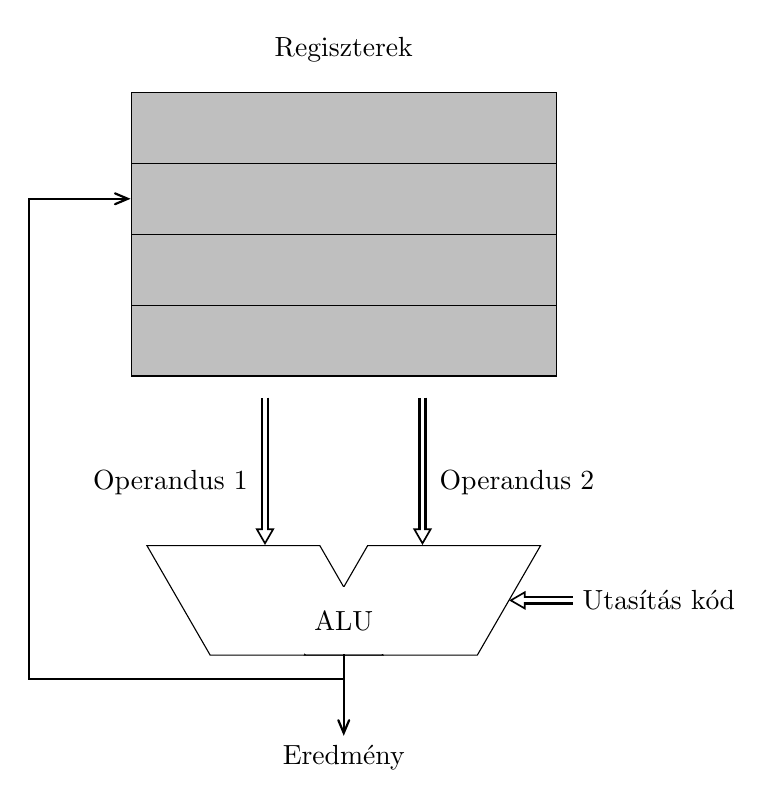
\begin{tikzpicture}
\tikzstyle{register}=[rectangle,align=center,draw,fill=lightgray,inner sep=0.2cm,text width=50mm,text height=5mm]
\tikzstyle{placeholder}=[rectangle,align=center,draw,fill=white,text height=6mm,color=white]
\tikzstyle{trapezoid_left}=[trapezium, draw, minimum width=3cm,trapezium left angle=120, trapezium right angle=60]
\tikzstyle{trapezoid_right}=[trapezium, draw, minimum width=3cm,trapezium right angle=120, trapezium left angle=60]
\node (reg_felirat) at (2,1){Regiszterek};
\node (eredmeny_felirat) at (2,-8){Eredmény};
\draw[-angle 45,thick] (2,-6.5)--(eredmeny_felirat);
\node[placeholder] (reg4_1)  at (1,-3){};
\node[placeholder] (reg4_2)  at (3,-3){};
\node[register] (reg1) at (2,0){};
\node[register] (reg2)  at (2,-0.9){};
\node[register] (reg3) at (2,-1.8){};
\node[register] (reg4)  at (2,-2.7){};
\node[trapezoid_left] (alu1) at (1,-6) {};
\node[trapezoid_right] (alu2) at (3,-6) {};
\node[placeholder] at (2,-6.254) {ALU};
\node (operandus2)  at (4.2,-4.5){Operandus 2};
\node (operandus1)  at (-0.2,-4.5){Operandus 1};
\node (ALU) at (2,-6.27){ALU};
\node (opcode) at (6,-6){Utasítás kód};


\tikzstyle{vecArrow} = [thick, decoration={markings,mark=at position
   1 with {\arrow[semithick]{open triangle 60}}},
   double distance=1.4pt, shorten >= 5.5pt,
   preaction = {decorate},
   postaction = {draw,line width=1.4pt, white,shorten >= 4.5pt}]

  \draw[vecArrow] (reg4_1) to (alu1);
  \draw[vecArrow] (reg4_2) to (alu2); 
  \draw[vecArrow] (opcode) to (4.1,-6); 

\draw[-angle 45,thick](2,-7)--(-2,-7)--(-2,-0.9)--(reg2);

\end{tikzpicture}
\caption{Egy utasítás végrehajtásának vázlata}
\label{fig:alu}
\end{figure}

\paragraph{Arithmetic Logic Unit (ALU)} Aritmetikai és Logikai Egység, azaz a processzor műveletvégző egysége. Egyszerű, aritmetikai (összeadás, szorzás, stb\ldots), logikai (ÉS, VAGY, stb\ldots) műveletek elvégzésére alkalmas logikai áramkör. Egy ALU jellemzően egyszerre egy műveletet képes elvégezni, jellemzően maximum két operandussal (bemenő értékkel). Az operandusok mellett szüksége van arra az információra is, hogy milyen műveletet kell elvégeznie az operandus(ok)on, ami szintén egy bináris kódként kap meg, ez az utasítás kód, angolul operation code (OpCode). Az ALU-nak kimenete egyrészt az elvégzett művelet eredménye, illetve emellett még beállít úgynevezett Flag-eket (a processzorban lévő, egy bites értékeket tároló egységek), amikkel jelezheti például, hogy az elvégzett művelet eredménye nagyobb, mint a processzor által kezelhető maximális méretű szám (azaz ``túlcsordul''), vagy éppen nulla. A Flag-ek beállítása azért fontos, mert az utasítások egy része eltérő módon viselkedik a Flag-ek értékének függvényében, így megvalósíthatóak például feltételes ugrások. Azt, hogy az ALU mekkora méretű adatokon tud műveleteket végezni, a CPU szóhossza határozza meg.
  \paragraph{Regiszterek} a CPU-n belül adattárolásra alkalmasak. Méretük általában megegyezik a processzor szóhosszával, és viszonylag kevés (nagyságrendileg maximum néhányszor tíz darab) található belőlük egy CPU-ban, pontos számuk a konkrét architektúrától függ. Jelentőségük abban áll, hogy a bennük tárolt adatok nagyon gyorsan (jó közelítéssel azonnal) elérhetőek, ellentétben az operatív memóriában, vagy a háttértáron tárolt adatokkal. Ennek következtében az ALU egy-egy művelet operandusait jellemzően egy-egy regiszterből veszi, illetve a művelet eredménye is egy regiszterbe íródik be (később látható lesz, hogy erre vannak egyéb megoldások, de az alapelv a legtöbb architektúra esetén azonos). Ha azt szeretnénk, hogy a processzor egy operatív memóriában lévő adategységen végezzen műveletet, akkor azt először be kell másolnia egy regiszterbe (amire rendelkezésre áll egy vagy több külön utasítás), majd ez után a regiszterbe lévő adaton végrehajtható a kívánt utasítás (például egy összeadás). Ha szükséges, a művelet eredményét szintén egy külön utasítással írhatjuk ki az eredmény-regiszterből az operatív memóriába. Egy speciális regiszter a \textbf{programszámláló} a következő végrehajtandó utasítás memóriacímét tárolja. Gyakran egy kijelölt regiszter felelős a Flag-ek tárolásáért is, ilyenkor ennek egyes bitjei külön-külön értelmezendőek. 
  \paragraph{Control Unit (CU)}, azaz vezérlőegység. Feladata az egyes utasítások végrehajtása során a többi komponens vezérlése, ennek megfelelően felolvassa a soron következő utasítást az operatív memóriából, megállapítja, hogy \emph{mit} kell csinálni (ha aritmetikai művelet, akkor ez lesz az ALU által megkapott OpCode), mik a paraméterek (ha vannak), azaz mely regiszterek értékét kell az ALU-nak felhasználnia operandusként, és hova (melyik regiszterbe) kerüljön az eredmény, ha van. Ha nem olyan utasításról van szó, amelyek az ALU hajt végre, hanem például memóriába írásról van szó, vezérli az ezt végrehajtó egységet is. Az utasítások végrehajtása végén növeli a programszámláló értékét, így a processzor az egyes utasításokat szekvenciálisan (sorban, egymás után) hajtja végre (lehetőség van azonban a programszámláló értékét egyéb módon is állítani, így befolyásolni az utasítások végrehajtásának sorrendjét, például létezik olyan utasítás, ami a programszámláló-regiszterbe ír egy értéket, az ilyen utasítást \textbf{ugró utasításnak} nevezzük).

\subsubsection{Memória}
Az (operatív) memória, amit szokás RAM-nak is nevezni (bár ez alapvetően mást jelent) a program által a futása során felhasznált adatok tárolására szolgáló egység. Ide tartoznak olyan adatok, amiken műveleteket kell végezni és a műveletek eredményei is, hiszen a processzorok regiszterkészletének mérete korlátos, egyáltalán nem biztos, hogy az összes, futás során szükséges adat elfér benne. Ugyanakkor lehet, hogy bizonyos adatokra csak a futás eltérő szakaszaiban van szükség, így nem is fontos minden adatot folyamatosan regiszterekben tárolni.

A számítógép az operatív memóriában az adatokat ``ömlesztve", különösebb struktúra nélkül tárolja, így az egyes adategységeket \textbf{memóriacímük} segítségével érhetjük el. A memóriacím egy pozitív egész szám, egy memóriában tárolt adategység (bájt) címe annyi, ahányadik bájt azt tárolja a memóriában. Természetesen gyakran használunk egy bájtnál nagyobb adategységeket is, ezeket az első bájtjuk címével, azaz \textbf{kezdőcímükkel} és \textbf{méretükkel} szokás címezni. 


Illusztrációképp szerepel \aref{memorydump}. ábrán egy alkalmas program segítségével megjelenített memóriatartalom. Az első oszlopban látható a sorok kezdőcíme, ezt követi 18 bájtnyi adat, majd a tárolt értékeknek megfelelő ASCII karakterek láthatók.
 
Fontos megjegyezni, hogy gyakran nem minden memóriacímhez tartozik fizikai memória, mivel a memóriacímek tetszőleges, a processzor szóhosszán ábrázolható nem negatív egész számok lehetnek, míg a számítógépekbe beépített fizikai memória mennyisége változhat, és jellemzően kisebb, mint a címtartomány mérete. Ez különösebb problémát nem okoz, mert az általunk tárgyalt esetekben az operációs rendszer végzi a memória kiosztását az egyes programok között, és gondoskodik róla, hogy azok csak megfelelő memóriacímeket használhassanak.
%\usepackage{graphics} is needed for \includegraphics
\begin{figure}[htp] 
\begin{center}
  \includegraphics[scale=0.5]{figures/memory_dump.png}
  \caption[Egy memóriakép]{Egy megjelenített memóriatartalom}
  \label{memorydump}
\end{center}
\end{figure}

% Memória használata: \TODO{}

\subsubsection{Háttértár}
A memóriáktól eltérően a háttértárak célja nagymennyiségű \textbf{adat tárolása}. Napjaink asztali számítógépeiben használt háttértárak tipikusan merevlemezek (más néven winchester, hard disk drive, rövidítve HDD) vagy SSD-k (solid state drive). Jellemzőjük a -- memóriákhoz viszonyított -- nagy méret és lassúság illetve az, hogy akkor is megőrzik az adatokat, ha számítógépet kikapcsoljuk/áramtalanítjuk. 


Egy HDD-n tárolt adat elérési ideje a memóriába már betöltött adatéhoz hasonlítva több nagyságrenddel is elmarad. (Számokkal illusztrálva: memóriábol olvasni kb. 0.7 ns, míg a háttértárról kb. 10 ms!) Ennek oka a hardver sajátosságában keresendő: egy winchester belsejében forgó lemezek hordozzák fizikailag az adatokat, és őket pásztázó fejek segítségével lehet írni vagy olvasni azokat. Ennek kompenzálására ezek az eszközök nem bájtonként címezhetők, hanem nagyobb egységeket kezelve úgynevezett \textbf{blokkos elérést} biztosítanak. Egy blokk mérete általában 4 KB és 1 MB közé esik, így valójában egy olvasással egyszerre több adathozzáférést is végrehajt, ezzel csökkentve az átlagos olvasási időt.
 
A manapság egyre terjedő SSD-k esetén az adathozzáférési idő kb. 0.1 ms. Ezek az eszközök nem tartalmaznak mozgó alkatrészeket, csupán a bennük található áramkörök jellemzői határozzák meg ezt a sebességet.


Fontos megjegyezni, hogy háttértáron tárolt adatokon közvetlen nem lehet műveleteket végrehajtani, előbb a szükséges részek memóriába helyezése szükséges.


\subsection{Gépi kód} 
A processzor által futtatott programot is a memóriában tároljuk, ennek megfelelően szintén binárisan kell reprezentálni, méghozzá úgy, hogy a processzor (azon belül is a Control Unit) ezt közvetlenül értelmezni tudja. A gyakorlatban ez azt jelenti, hogy az egyes utasításokat tároljuk binárisan kódolva, egymás után a memóriában. A processzor a programszámláló által mutatott helyről olvassa be az egyes utasításokat, majd végrehajtja őket (és természetesen közben a programszámláló értéke is változik). 

Sajnos annak, hogy a processzor által könnyen értelmezhető formában tároljuk a programot (azaz a végrehajtandó utasításokat) az az ára, hogy ezek ebben a formában egy ember számára nehezen értelmezhetőek, hiszen 1-esek és 0-k sorozatáról van szó. Az első részük jellemzően az utasítás kódját (OpCode) tárolja, majd további számjegyek kódolják a hozzá tartozó egyes paramétereket, amik lehetnek számok, vagy regiszterek kódjai. Az informatika hőskorában a programozók ilyen formában dolgoztak, közvetlenül gépi kódot írtak, ám ez nagyon lassú és nehézkes módszernek bizonyult (táblázatokból kellett kiolvasni a különféle utasításokhoz tartozó bináris számokat).

Ennek eredményeként hamar megoldást találtak a programkódok (ember által) könnyebben olvasható reprezentációjára, így ma már gyakorlatilag senkinek nem kell kézzel gépi kódot írnia.

\subsection{Assembly} 

Az első lépés a programkódok olvashatóbbá tételének irányába az Assembly nyelv bevezetése volt. Ez egy nagyon egyszerű megoldás, csupán arról van szó, hogy az egyes utasítások OpCode-ját valamilyen, a funkciójukra utaló, 2-4 betűs betűkóddal (mnemonic), a paraméterek esetében pedig a regiszterek kódját szintén valamilyen rövid névvel helyettesítjük (ha a paraméter értéke számként értelmezendő, a számot közvetlenül leírhatjuk).

Az alábbiakban szerepel egy egyszerű Assembly példakód, melyről feltételezhetjük hogy egy nagyobb program részlete:
% \TODO{esetleg labelekrol irni}
\asmlisting
\lstinputlisting {codeexamples/asmexample.asm}

A példa első sorában egy úgynevezett \textbf{címke} szerepel, aminek a jelentősége, hogy ennek segítségével lehet a program meghatározott pontjaira hivatkozni. Ez tulajdonképpen egy memóriacímet jelent, leginkább a programozót segíti az olvashatóság javításával.


A második sorban egy \textbf{mozgatás} utasítás áll, mely betölti a 45 számértéket az \texttt{ax} regiszterbe.


A harmadik sorban egy \textbf{összeadás} szerepel. Az \texttt{ax} regiszterben szereplő 45-höz hozzáadja a \texttt{bx} regiszter tartalmát. Ekkor a két operandus közül az első felülíródik és ebbe kerül be az eredmény.

A negyedik sorban egy \textbf{összehasonlítás}t végzünk, ahol a kapott összegre vizsgáljuk, hogy milyen viszonyban áll a 100 konstanssal. Ez az utasítás beállít és kitöröl bizonyos flag-eket az összehasonlítás eredményének megfelelően. 
 
Végül az ötödik sorban az összehasonlítás eredményét felhasználva \textbf{ugrást} hajtunk végre a kódban az eleje: címkével ellátott pontra, ha az \texttt{ax}-ben tárolt érték nagyobb vagy egyenlő mint 100.
 

Megfigyelhető, hogy a leírt kód információtartalma megegyezik a gépi kódéval, továbbra is egyenként, egymás után írjuk a processzor által végrehajtandó utasításokat, a különbség az, hogy valamivel könnyebben olvasható lesz a kód.

Annak, hogy az Assembly kód nagyon közel áll a gépi kódhoz, az az előnye, hogy nagyon könnyű gépi kódot előállítani belőle, egy igen egyszerű program (amit \textbf{Assembler}-nek hívunk) képes erre. Ebből következik, hogy ez a megoldás már az informatika fejlődésének korai szakaszában megjelent, nagyon sokáig ilyen formában íródtak a programok.

Mivel az Assembly-utasítások egyértelműen megfeleltethetőek a processzor gépi utasításainak, fontos megjegyezni, hogy mivel az egyes processzorarchitektúrák eltérő utasítások végrehajtását támogatják, \emph{nem létezik egységes Assembly nyelv, hanem az egyes architektúráknak van Assembly-nyelve}, amelyek természetesen hasonlítanak egymásra, de nem azonosak.

Sajnos nagyobb, bonyolultabb programok fejlesztésénél az Assembly-kód gyorsan áttekinthetetlenné válik, ezért manapság nem igazán használjuk, a helyét magasabb szintű nyelvek vették át. Vannak azonban esetek, amikor nagyon fontos az elkészített program mérete és hatékonysága (vagy azért, mert egy nagyon egyszerű, kis teljesítményű eszközre fejlesztünk, vagy épp ellenkezőleg, nagyon gyors működést várunk el), ilyenkor még manapság is szokás a kódot (vagy inkább annak kritikus részeit) Assembly nyelven írni, mivel így tudjuk a legközvetlenebbül befolyásolni a processzor működését.

 

\subsection{Magas szintű nyelvek}

\subsubsection{Motiváció}

Az Assembly nyelvek használata ugyan megoldotta a gépi kód ember számára nehéz olvashatóságának problémáját, azonban a programok egyre növekvő komplexitására nem jelentett igazi megoldást. Az Assembly kód a legtöbb esetben túlságosan közvetlenül írja le a programunk működését, hiszen explicite meg kell adnunk az egyes utasításokat, azok pontos paraméterezésével együtt, ugyanakkor a programozó számára például gyakran nem fontos, hogy egy művelet eredménye melyik regiszterbe kerül, vagy egyáltalán regiszterbe kerül-e, esetleg az operatív memóriába, illetve ha a memóriába kerül, akkor pontosan hova (milyen címre), így könnyű ``elveszni a részletekben''.

Hasznos lenne egy olyan nyelvet használni, amiben a programokat absztraktabb, azaz elvontabb módon, tömörebben, lényegre törőbben írhatnánk le, csak a működés szempontjából lényeges dolgokkal kellene foglalkoznunk a programok írása közben. Ezzel együtt pedig rövidebb, áttekinthetőbb, és jobban strukturált (így később sokkal könnyebben megérthető, karbantartható) kódot kaphatnánk. 

A C, illetve az ennek bázisán kifejlesztett C++ nyelv ilyen, úgynevezett \textbf{magas szintű nyelv}.
Fontos megjegyezni, hogy \emph{egy programozási nyelv ``magas szintű'', vagy ``alacsony szintű'' mivolta erősen kontextus függő}. Az Assembly-hez képest a C nyelv például magas szintűnek tekinthető, mivel sokkal absztraktabb módon, a hardver sajátosságaival kevésbé foglalkozva írható le benne egy adott program, ugyanakkor léteznek a C-nél ``magasabb szintű'' nyelvek is, amik még absztraktabb leírást tesznek lehetővé, még jobban elfedik a hardveres megvalósítás részleteit. Ilyen például a Java nyelv, így a Java és a C kontextusában vizsgálva a C alacsony szintű nyelvnek számít, míg a Java magas szintűnek. A C++-t általában valamivel magasabb szintű nyelvnek szokás tekinteni, mint a C-t, de alacsonyabb szintűnek, mint a Java-t. Látható, hogy ezek a fogalmak nem teljesen egzaktak, mi a továbbiakban a C-re és a C++-ra is mint magas szintű nyelvre fogunk hivatkozni.

\subsubsection{Fordító}
Sajnálatos módon annak, hogy a programunkat egy magas szintű nyelven írjuk le, hátránya is van. Az Assemblytől eltérően (ami gyakorlatilag a gépi kódnak az olvashatóbb alakban leírását jelenti) egy magas szintű, például C nyelvű \textbf{forráskód} szemantikailag (jelentésében) nagyon távol állhat az általa leírt funkciót megvalósító gépi kódtól. 
A gépi kód (ahogy az Assembly is) a processzor által végrehajtható utasításokat tartalmaz egymás után, míg egy magasabb szintű forráskód jellemzően bonyolultabb (csak több gépi utasítással megvalósítható) műveleteket, vezérlési szerkezeteket, illetve függvényhívásokat (ezekre részletesebben később fogunk kitérni).
Ez azzal jár, hogy a forráskódból gépi kódot előállítani messze nem olyan egyszerű feladat, mint az Assembly nyelvnél, sokkal bonyolultabb, több logikát tartalmazó szoftver szükséges hozzá.

\textbf{Fordítónak} (compiler) nevezzük azokat a programokat, amik valamilyen magas szintű forráskódból alacsonyabb szintű, jellemzően (de nem mindig) gépi kódot állítanak elő, magát a folyamatot pedig fordításnak. A fordítás általában nem egyértelmű folyamat, egy bizonyos forráskódból több, funkcionálisan azonos (azaz ``ugyanazt csináló''), de különböző gépi kód is előállítható, hiszen egy absztrakt módon megfogalmazott műveletet adott esetben több, eltérő utasítássorozat is megvalósíthat. Azt, hogy a fordító egy bizonyos esetben pontosan milyen gépi kódot állít elő, közvetlenül ugyan nem határozhatjuk meg (lássuk be, pont azért használunk valamilyen magas szintű nyelvet, mert nem szeretnénk ilyesmivel foglalkozni), ugyanakkor közvetett módon befolyásolhatjuk, megmondhatjuk például a fordítónak, hogy gyorsan működő kódot szeretnénk (futási időre optimalizálás), vagy inkább kevés utasításból állót (kód méretére optimalizálás), esetleg kevés memóriát felhasználót (memóriahasználatra optimalizálás), a fordító pedig igyekszik a lehetőségeihez mérten ilyen gépi kódot létrehozni.

Az Assembly-hez képest komoly különbség a magasabb szintű nyelvek esetén, hogy ezek szabványosak, tehát (mivel a cél a hardverfüggő részletek elfedése) a forráskód szintaktikája (lásd később) nem függ attól, hogy a belőle fordított gépi kódot milyen processzorarchitektúrán fogjuk futtatni, így nincs szó például C nyelvekről, csak C nyelvről. Ha különböző processzorarchitektúrákon szeretnénk egy bizonyos forráskódból készült gépi kódot futtatni, akkor nyilvánvalóan különböző gépi kódra van szükségünk, erre általában az a megoldás, hogy az egyes architektúrákra különböző fordítóprogramokkal fordítjuk le a forráskódot.

Az idő előrehaladtával a fordítóprogramok folyamatosan fejlődnek, egyre intelligensebbek lesznek, egyre hatékonyabb gépi kódot lesznek képesek előállítani. Korábban gyakran szükség volt a teljesítménykritikus kódrészletek Assembly-ben történő megírására, ma már néhány igen szélsőséges esettől eltekintve a fordítók jobb minőségű (hatékonyabb) gépi kódot tudnak előállítani, mint egy hozzáértő programozó Assembly-ben, így erre ritkán van szükség.

Megjegyzés: a magas szintű nyelven megírt programok futtatására nem az egyetlen megoldás a fordítóval gépi kódú program előállítása, majd annak futtatása. Léteznek úgynevezett \textbf{interpretált nyelvek}, amelyeket nem fordítunk gépi kóddá, hanem egy \textbf{interpreter} (értelmező) nevű program sorról sorra feldolgozza (``értelmezi'') a forráskódot, és az egyes utasításokat rögtön végre is hajtja. Ilyen nyelv például a régen oktatási célra igen elterjedt, ma már ritkán használt BASIC. Általában elmondható, hogy egy interpretált nyelven megírt program az interpreter folyamatos működése miatt kisebb teljesítményű (lassabb) lesz, mint ha egy fordítható nyelven írnánk meg, bináris gépi kóddá fordítanánk és azt közvetlenül futtatnánk, ezért általános programozási nyelvként ezek gyakorlatilag kiszorultak, azonban léteznek olyan speciális alkalmazási területek, amikor alkalmazunk interpretereket.

\subsubsection{Szintaktika} 
A programozási nyelvek -- akárcsak a természetes nyelvek -- rendelkeznek szintaxissal, azaz nyelvtannal, nyelvtani szabályokkal. Két részre bontható fel:
\begin{itemize}
  \item \textbf{absztrakt szintaxis}: definiálja, hogy mit képes a nyelv kifejezni
  \item \textbf{konkrét szintaxis}: meghatározza, hogy az egyes nyelvi elemeket hogyan kell jelölni 
\end{itemize}

A C nyelvet felhasználva egy konkrét példán keresztül mutatjuk be, mit is jelent ez a két fogalom. Tegyük fel, hogy egy olyan egyszerű programot készítünk, ami megszámolja, hogy hány szóköz karakter van egy szövegben. Ekkor szükségünk van egy \emph{egész szám}ra, amivel ezt az értéket reprezentálni tudjuk. Az alábbi C nyelvű kódsort leírva fejezhetjük ki, hogy legyen egy \texttt{szokozokSzama} nevű egész számunk.

\clisting
\lstinputlisting{codeexamples/declaration.c}
A példában az absztrakt szintaxis teszi lehetővé, hogy egész számokat tudjunk leírni. A kapcsolódó konkrét szintaxis pedig a fenti kódsor. Ennek részei:
\begin{itemize}
  \item az \texttt{int} kulcsszó, mert ezzel jelöljük, hogy egy egész számot (integer) szeretnénk tárolni
  \item a neve, ami most \texttt{szokozokSzama}
  \item a sorvégi \texttt{;} karakter, mivel a nyelvtani szabályok előírják, hogy minden egyes utasítást ezzel kell lezárni
\end{itemize}


\subsubsection{C nyelv}
A C nyelvet 1969 és 1973 között fejlesztették ki az Egyesült Államokban, az ATT Bell Labs-nál. Azóta minden idők legszélesebb körben használt programozási nyelve lett, a legkisebb mikrovezérlőktől a legnagyobb szuperszámítógépekig futtathatunk C nyelven írt programokat, köszönhetően annak, hogy rengeteg féle processzorarchitektúrához készült C fordító.

A ma használt modernebb (és magasabb szintű) nyelvekhez képest valamivel közvetlenebb kontrollt enged meg a hardver felett és ezért általános célú, PC-s alkalmazásokat már viszonylag ritkán szokás C-ben írni, de ettől még igen elterjedt például beágyazott rendszerekben, vagy olyan, teljesítménykritikus szoftvereknél, mint a különféle hardverek illesztőprogramjai (driverek).

Ezen tulajdonsága miatt különösen alkalmas a programozás oktatására is, nem véletlen, hogy mi is ezt (illetve bizonyos esetekben a C++-t, de mint később látni fogjuk, ez nem jelent nagy különbséget) választottuk a gyakorlati példáinkhoz. 



\subsubsection{C++ nyelv}
Bjarne Stroustrup dán informatikus tervezte 1983-ban, azóta rengeteg, egyre modernebb szabványa jött létre. Az előzőekben röviden bemutatott C nyelv hiányosságait és kényelmetlen megoldásait igyekszik orvosolni. Egy nyelv problémái például az alábbiakból adódhatnak:
\begin{itemize}
  \item szintaxis bonyolultsága, kényelmetlen használata
  \item hiányos elemkészlet
  \item hatékonysági kérdések
  \item programozási irányelvek (paradigmák) támogatása
\end{itemize}

Távolról szemlélve, pár kivételtől eltekintve igaz, hogy a C nyelv egy részhalmazát képezi a C++-nak. Ez utóbbiról elmondható, hogy modernebb nyelvi elemeket és megoldásokat ad a C-hez, azonban ez valamelyest csökkenti a teljesítményét a belőle lefordított kódnak. Sok alkalmazási területen viszont a C++ kínálta eszközkészletért nem nagy ár az ezzel vesztett teljesítmény. Későbbiekben ezek közül a különbségek közül néhánnyal részletesebben foglalkozunk.
 

\chapter{A C nyelv}
\label{02_c_nyelv}

Ezen fejezet témája a C nyelv nyelvtana lesz.

A következőben egy rövid forráskód-részleten keresztül mutatjuk be, hogy hogy néz ki egy C program. 


\clisting
%\begin{landscape}
\label{first_c_example}
%----------------------------------------------------------------------------
\lstinputlisting{codeexamples/first_c_example.c} 
%\end{landscape}

Az első soban egy úgynevezett \textbf{preprocesszor direktíva} található. A forráskód lefordítása során a tényleges fordítás előtt egy másik program(rész) is feldolgozza azt, ez a \textbf{preprocesszor}. A forráskódban azok a sorok, amelyek a preprocesszornak szólnak, jellemzően \#-al kezdődnek, ezeket feldolgozza, jellemzően valamilyen transzformációt hajt végre a forrásfájlon, majd ezt követően kerül sor annak tényleges lefordítására.

Jelen esetben egy \textbf{include direktívával} találkozunk, ez azt jelenti, hogy forráfájlunkban valamely másik fájl tartalmát is fel szeretnénk használni, ez most az stdio.h fájl, ami a szöveges I/O műveleteket támogató függvények deklarációját tartalmazza. A preprocesszor \emph{az include direktíva helyére ideiglenesen beilleszti a megjelölt fájl teljes tartalmát}, így a fordító ezt is benne fogja találni a forrásfájlunkban.

Léteznek egyéb preprocesszor direktívák is, ezekről később ejtünk szót.

A 3. és 4. sor egy-egy \textbf{függvénydeklarációt} tartalmaz. A C nyelvben a forráskódot úgynevezett \textbf{függvényekbe} szervezzük, csoportosítjuk, egy függvény általában egy bizonyos funkciót ellátó kódot fog össze. Ezeket azért hívjuk függvényeknek, mert futásuk során valamilyen \textbf{paraméterek} függvényében visszaadnak valamilyen \textbf{értéket} (amit visszatérési értéknek hívunk), hasonlóan a matematikában megszokott függvényekhez. Természetesen nem csak matematikai függvényekről lehet szó, bármilyen módon előállíthatják a visszatérési értéket, sőt, olyan függvény is elképzelhető, amelyik semmilyen visszatérési értékkel nem rendelkezik, ugyanígy a paraméterek száma is lehet 0, vagy akár tetszőlegesen sok.

A 3. és 4. sor csupán deklaráció, tehát a 3. sor jelentése a következő: ``valahol a kódban lesz majd egy olyan kódrészlet (egy függvényként), amelynek a paramétere két egész szám (angolul integer, ezt rövidítve a C nyelvben \textbf{int}), a visszatérési értéke szintén int, azaz egész szám, míg a neve ``osszead''. A deklarációt, mint minden C nyelvű utasítást egy pontosvessző zárja. Fontos, hogy ez a sor nem tartalmazza az ``osszead'' nevű függvény \textbf{implementációját}, azaz nem írja le, hogy a függvény ``mit is csinál'', csupán azt határozza meg, hogy milyen típusú paramétereket lehet neki átadni, illetve milyen típusú lesz a visszatérési értéke. A funkcionalitást leíró rész, azaz az implementáció, amit \textbf{függvénydefiníciónak} is nevezünk, később következik.

Hasonlóan, a 4. sorban található deklaráció jelentése: ``valahol a kódban (akár egy másik fájlban!) lesz majd egy függvény, aminek 0 darab paramétert lehet átadni és egy egész számot (int) ad vissza, neve pedig ``misztikusFuggveny''.

A 6. sorban egy úgynevezett megjegyzés, avagy \textbf{komment} található. Ezek olyan részek egy forráskódban, amelyeket a fordító figyelmen kívül hagy, funkciójuk csupán a kód működésének magyarázata, a megértés segítése. Azt, hogy egy kódsor kommentként értelmezendő, úgy jelezhetjük, hogy két darab / jelet teszünk az elejére. Forráskódunkban azokat a részeket, amik nem triviálisak, amelyek működése félreérthető, vagy sokat kell gondolkodni a megértéséhez, célszerű kommenttel ellátni, és tömören, lényegre törően leírni, hogy mi is történik ott és miért. Ennek azért van jelentősége, mert bár lehet, hogy mi értjük a saját magunk által írt kódot, de ha olyasvalakinek kell olvasnia és megértenie, aki nem ismeri (és ebbe mi is beletartozunk, ha például hónapok elteltével veszünk elő egy kódrészletet), nagy könnyebbséget jelent némi magyarázó szöveg. Fontos azonban, hogy ne írjunk felesleges kommenteket triviális kódrészletekhez, mert a megértést ebben az esetben érdemben nem segíti, ugyanakkor ha adott esetben módosítani kell a kódot, akkor többletmunkát jelent a kommentek módosítása is.

Az 7. sor egy \textbf{függvénydefiníció} kezdete, az úgynevezett fejléc. Itt a ``main'' nevű függvény definíciója kezdődik. A ``main'' egy speciális függvény, ugyanis a továbbiakban is minden programunkban lennie kell egynek, és amikor egy programot elindítunk, az a ``main'' függvénnyel kezdi a futását, ezt az operációs rendszer hívja meg (ezt \textbf{belépési pontnak} hívjuk). Paramétere jelen esetben nincs (ez nem mindig van így), a visszatérési értéke pedig egy egész szám, ami a gyakorlatban egy hibakód, ezzel lehet jelezni az operációs rendszer felé, hogy a program rendben lefutott, vagy esetleg valamilyen hiba történt. 

A függvény fejléce után kapcsos zárójelek között következik a \textbf{függvénytörzs}, ami a függvény meghívása során végrehajtandó kódot tartalmazza. A függvénytörzs sorai egymás után fognak végrehajtódni. 

Jelen esetben az 8-10. sor között három darab \textbf{változódeklaráció} található. Ezekkel azt fejezzük ki, hogy a függvénytörzsben használni fogunk három darab \textbf{változót}, amik gyakorlatilag olyan ``rekeszek'', amikben adategységeket tárolhatunk. Az egyes változók tartalma mögött az operatív memória egy-egy tartománya áll, tehát az értékek ott tárolódnak, azonban hogy milyen címen és milyen méretű (hány bájtos) memóriaterületen, azzal általában nem kell foglalkoznunk, a nyelv elfedi előlünk (ez alól természetesen majd lesznek kivételek). Az egyes változók típusa határozza meg egyrészt a változó tárolására használt memóriaterület méretét, másrészt útmutatást nyújt azzal kapcsolatban, hogy a benne tárolt adatok hogyan értelmezendőek. Esetünkben mindhárom \textbf{int}, azaz (előjeles) egész szám típusú, nevük pedig a, b és osszeg. Sajnos a C nyelv kellemetlen tulajdonsága, hogy nincsen rögzítve az alapvető típusok pontos mérete, de azt például tudjuk, hogy az int típus mérete jellemzően megegyezik azon processzorarchitektúra szóhosszúságával, amire fordították. Ezt sajnos tovább bonyolítja az, hogy például az Intel x86-64 architektúrájú processzorok (amelyek szóhosszúsága 64 bit) képesek olyan programokat is futtatni, amiket a régebbi, 32 bites szóhosszúságú Intel x86 architektúrára fordítottak, így ezeket a programokat hiába futtatjuk 64 bites processzoron, az int változók mérete továbbra is 32 bites lesz, ami pedig nyilvánvalóan meghatározza a bennük tárolható számok maximális (illetve minimális, hiszen negatív számokat is tárolhatunk) méretét.

\emph{A változók deklarációjakor még nem tudhatjuk, hogy ezekben a ``rekeszekben'' mi van, mi a számok értéke, jellemzően valamilyen véletlenszerű értéket vesznek fel} (a memóriában valaki által korábban ``ott felejtett'' érték, azaz \textbf{memóriaszemét}). Figyeljük meg, hogy ezeket a sorokat is egy-egy pontosvessző zárja.

A 12. és a 13. sor egy-egy \textbf{értékadást} tartalmaz. Jelentésük: ``az 'a' változó értéke legyen 5'', illetve ``a 'b' változó értéke legyen 3''. Mint minden utasítást, ezeket is pontosvessző zárja. Ha egy értékadás célja az, hogy egy változót valamilyen kezdeti értékkel lásson el (azaz hogy memóriaszemét helyett valamilyen értelmes, később használható értéket tároljon), a műveletet a változó \textbf{inicializálásának} is nevezhetjük.

A 15. sorban szintén egy értékadás található, itt azonban az ``osszeg'' változónak nem egy konstans értéket adunk, hanem azt írtuk utána, hogy ``osszead(a, b)''. Ez azt jelenti, hogy hívjuk meg (\textbf{függvényhívás}) az ``osszead'' függvényt, amit korábban deklaráltunk, és adjuk át neki első paraméterként az 'a' változót (aminek értéke ezen a helyen 5), illetve második paraméterként a 'b' változót, ami itt most 3 értéket vesz fel, majd azt az értéket, amivel ez visszatér, adjuk értékül az ``osszeg'' változónak.

Fontos, hogy ezen a ponton a fordító (mivel sorról sorra megy végig a forráskódon) nem tudja, hogy mit is csinál az ``oszead'' függvény, lehet, hogy összeadja a két paraméterét, és azt adja vissza, lehet, hogy elosztja az elsőt a másikkal, de az is lehet, hogy minden esetben 42-t ad vissza. A fordító csupán azt tudja, hogy létezik egy olyan függvény, aminek két egész számot lehet átadni paraméterként és egy egész szám a visszatérési értéke, hiszen a program első sorában lévő deklaráció csupán ennyi információt tartalmaz, ez azonban pont elég ahhoz, hogy ezt a kódot le tudja fordítani.

A 17. sor a main függvény \textbf{visszatérési utasítását} tartalmazza. Ez azt jelenti, hogy ha idáig eljut a program futása, akkor a main függvény térjen vissza, 0 visszatérési értékkel. Mivel a main függvény egy speciális függvény, amit az operációs rendszer hívott meg a program elindításakor, ez azt fogja jelenteni, hogy a program futása véget ér, és az operációs rendszer a futás eredményeként hibakódként a 0-t kapja, ami azt jelenti, hogy nem történt semmilyen hiba, a program rendben lefutott.

A 18. sorban a main függvény törzsét lezáró kapcsos zárójel van, a C nyelv szintaktikája előírja, hogy minden függvénytörzset egy ilyennel zárjunk le. 

A 20. és 21. sor szintén egy kommentet tartalmaz, ezúttal a másik lehetséges jelölést alkalmazva. Ha egy szövegrészt /*-el kezdünk és */-el fejezünk be, akkor a közöttük lévő teljes szöveg kommentként értelmeződik és nem szükséges az összes sor elejére a //-t kitenni. Ez akkor hasznos, ha hosszú, sok soros kommentet szeretnénk írni. 

A 22. sorban kezdődik az ``osszead'' függvény definíciója, szintén a fejléccel. Ez gyakorlatilag a deklaráció megismétlése, ahhoz képest többletinformációt nem hordoz (a deklarációra csak azért van szükség, mert ez a függvény a main függvény után helyezkedik el a kódunkban, így ahhoz, hogy a main függvény fordítható legyen, annak fordításakor a fordítónak már tudnia kell róla, hogy valahol később lesz egy ilyen nevű, paraméterezésű és visszatérési típusú, azaz röviden ilyen \textbf{szignatúrájú} függvényünk, ezt a technikát \textbf{elődeklarációnak} hívjuk).

Az ``osszead'' függvény függvénytörzse (amelyet egy nyitó kapcsos zárójelnek kell megelőznie) két soros. 

A 24. sor egy újabb függvényhívás (azaz egy, a main() függvényből meghívott függvényből újabb függvényeket hívhatunk meg, és ezt tetszőleges mélységig folytathatjuk), jelen esetben a misztikusFuggveny nevű függvényt hívjuk meg. Paramétert nem adunk át neki, mivel a függvény deklarációja megmondja, hogy ez a függvény nem fogad paramétereket és \emph{egy függvény meghívásakor mindig a deklaráció által előírt mennyiségű és típusú paramétereket kell átadnunk}. A függvénynek ugyanakkor van egy int típusú visszatérési értéke, ezt azonban nem kell feltétlenül felhasználnunk, meghívható a függvény anélkül, hogy a visszatérési értékét bárminek értékül adnánk, és le is fog futni, ha van valamilyen hatása a futásának, az meg fog történni, majd a visszatérési értéke egyszerűen elveszik.

A 26. sor egyben az osszead függvény visszatérési utasítása is, azt jelenti, hogy ``a függvény visszatérési értéke legyen az első paraméter (operandus1) és a második paraméter (operandus2) összege''. Tehát a függvény a nevének megfelelően összeadja a két paraméterként kapott egész számot, és az eredményt adja vissza, tehát a main-ben meghívva az ``osszeg'' változó értéke a 15. sorban 8 lesz. Az ``osszead'' függvény törzsét is kapcsos zárójel zárja.

A 29. sor egy újabb preprocesszor direktívát tartalmaz, láthatjuk, hogy kettős kereszt (hashmark) áll a sor elején. Ez pedig a \textbf{define direktíva}. Több esetben is használható, mi most egy konstanst definiálunk vele, aminek a példában látható szintaktikával a neve TOMB\textunderscore HOSSZ, értéke pedig 10. A direktívát a preprocesszor úgy kezeli, hogy a kód további részében a definiált kulcsszót (TOMB\textunderscore HOSSZ) mindenhol kicseréli az utána írt értékre (10-re). Nem csak számot definiálhatunk így, hanem bármilyen szöveget, ennek egészen bonyolult alkalmazásai lehetnek, igen összetett logikákat lehet define-okkal ``összetrükközni'', azonban mint azt később látni fogjuk, ez bizonyos esetekben veszélyes lehet, így sokszor érdemes egyéb megoldást keresni helyette.

Amire most mi használjuk, arra viszont tökéletesen megfelel, később az így definiált konstanst (TOMB\textunderscore HOSSZ) hasonlóan kezelhetjük, mint egy egész típusú változót, annyi különbséggel, hogy értéket nem adhatunk neki, és nem szabad elfelejtenünk, hogy a behelyettesítés még a forráskód tényleges lefordítása előtt történik, tehát ahova mi azt írjuk, hogy TOMB\textunderscore HOSSZ, ott a fordító azt fogja látni, hogy 10. Mégis igen hasznos ilyen formában definiálni értékeket, egyrészt azért, mert ``beszédesebbé'' teszik a kódot, mint ha közvetlenül számokat írnánk bele, másrészt segítik a karbantartását is, hiszen ha később kitaláljuk, hogy az az érték, amire most TOMB\textunderscore HOSSZ néven gondolunk legyen 10 helyett például 20, akkor elég egy helyen, a define direktívánál átírni, így kevesebb az extra munka, kevesebb a hibalehetőség.

A 31. sorban a misztikusFuggveny definíciója kezdődik, hasonlóan, mint az osszead függvénynél, a fejléccel.

A 33. sorban egy ismerős kifejezést látunk, ami egy változódeklarációhoz hasonlít, azonban a változó neve után egy szögletes zárójelben az áll, hogy TOMB\textunderscore HOSSZ. Az előbb leírt módon, mivel a TOMB\textunderscore HOSSZ egy preprocesszor direktívával definiált konstans, a preprocesszor a helyére 10-et fog behelyettesíteni, azaz a fordítás pillanatában a változó neve után 10 fog állni a szögeletes zárójelben. Ezzel a szintaktikával azt fejezhetjük ki, hogy egy tömböt szeretnénk deklarálni. A \textbf{tömb} egy olyan \textbf{adatstruktúra}, ami \emph{azonos típusú változókból, a memóriában folytonosan (egymás után) tárol} valahány darabot. Azt, hogy hány darabot tárol, a tömb \textbf{elemszáma} határozza meg, és ez az, amit a tömb deklarációjakor a szögletes zárójelbe írunk.

Jelen esetben egy olyan tömböt deklarálunk, aminek a neve ``szamok'', és TOMB\textunderscore HOSSZ darab (azaz 10 darab) int típusú (azaz előjeles egész) értéket tárol.

Természetesen a tömb elemeit el kell érnünk valahogyan, tehát hivatkozni kell rájuk, hasonlóan, mint az egyes változókra. Annyiban bonyolultabb a helyzet a tömbökkel, hogy amíg a változókat a nevükkel azonosíthatjuk a kódban, a tömbökre ez nem igaz, hiszen egy tömb több elemet is tárol, így valamilyen kiegészítő információ szükséges az egyes elemek eléréséhez. Erre az a megoldás, hogy ha egy tömb n. elemére szeretnénk hivatkozni, akkor a tömb neve után szögletes zárójelben oda kell írni n-et. Így a szamok nevű tömb 5. elemét például úgy érjük el, hogy szamok[5]. A szögletes zárójelbe írt értéket \textbf{indexnek}, az ilyen módon történő hivatkozást pedig \textbf{indexelésnek} nevezzük.

Fontos megjegyezni, hogy \emph{a tömbök elemei minden esetben 0-tól számozódnak}, tehát például ha a szamok tömb 10 elemű, akkor a legális indexek a [0..9] intervallumból kerülnek ki, így a szamok[10] módon hivatkozott érték már nem része a tömbnek, hanem egy azon kívüli, ismeretlen tartalmú és ``tulajdonosú'' memóriaterület, így arról olvasni memóriaszemetet fogunk, oda írni pedig a program (illetve speciális esetben az egész számítógép) működésének veszélyeztetésével jár, így szigorúan tilos. Ráadásul a szamok[10] kifejezés szintaktikailag helyes, így a fordító nem fog hibát jelezni rá, a hiba csak futás közben jelentkezik, így programok írásakor különösen figyelnünk kell arra, hogy tömböket csak legális indexekkel indexeljünk (azaz elkerüljük a \textbf{túlcímzést}, avagy \textbf{túlindexelést}).

A 34. és 35. sor egy-egy már korábban is látott változódeklarációt tartalmaz, annyi különbséggel, hogy most a deklarációval egy sorban megtörténik az egyik változó (magikusSzam) kezdeti értékének beállítása (inicializálás) is.

A 37. sorban egy \textbf{ciklus} kezdődik. A ciklus (hasonlóan egy függvényhez) két részből, a \textbf{ciklusfejből} és a \textbf{ciklustörzsből} áll.

A ciklusok \textbf{vezérlési szerkezetek}, és több fajtájuk van, ezek egyike a \textbf{for ciklus} (számláló ciklus), egy ilyennek a ciklusfeje látható a 37. sorban. A ciklusfej elején a for kulcsszó jelöli, hogy egy for ciklusról lesz szó, majd egy zárójelet követően a for ciklusok fejének (fejlécének) három, pontosvesszővel elválasztott, eltérő funkciójú része.

A nyitó zárójel után, de az első pontosvessző előtt található rész fut le először. A példánkban itt az i változó inicializálása történik, és a gyakorlatban ilyen jellegű kódot szokás ide írni, de természetesen bármilyen szintaktikailag helyes kód elhelyezhető itt.

A következő részben (a két pontosvessző között) egy feltételnek kell szerepelnie, azaz egy olyan kifejezésnek, ami valamilyen logikai értékre (igaz, vagy hamis) értékelődik ki. Később látni fogjuk, hogy a C-ben \emph{minden kifejezésnek van valamilyen logikai értéke}, de mégis praktikus valamilyen szemléletes, feltétel jellegű kifejezést írni ide, a kód könnyű megérthetőségét elősegítendő. A példában az ``i < TOMB\textunderscore HOSSZ'' kifejezés szerepel itt, ami logikai IGAZ értékű, ha i kisebb, mint TOMB\textunderscore HOSSZ, ha pedig egyenlő, vagy nagyobb, akkor logikai HAMIS értékű.

A for ciklus úgy működik, hogy a ciklustörzsben lévő kódot újra és újra végrehajtja, egészen addig, amíg a ciklusfej feltétel része logikai IGAZ értékű, ekkor befejeződik, és a kód végrehajtása a ciklus után folytatódik. 

A ciklusfej harmadik részébe írt kód a ciklustörzs minden egyes végrehajtása \textbf{után} hajtódik végre, ide most egy olyan utasítást írtunk, ami az i változó értékét növeli 1-el. 

Ennek megfelelően a teljes ciklus úgy fog működni, hogy először az i változó értékét 0-ra állítja, majd megvizsgálja a feltételt, ha IGAZ értékű, akkor végrehajtja a ciklustörzset, ezt követően végrehajtja a ciklusfej harmadik részét (azaz növeli az i változó értékét), ismét kiértékeli a feltételt, ha IGAZ, újra végrehajtja a ciklustörzset, újra növeli i-t, stb\ldots

Könnyen belátható, hogy mivel az i változó 0-ra inicializálódik és TOMB\textunderscore HOSSZ-nál kell kisebbnek lennie ahhoz, hogy a ciklustörzs lefusson, a ciklustörzs pontosan 10-szer fog lefutni, és i értéke eközben 0,1,2,\ldots,9 lesz, és jelen esetben pontosan ez a célunk.

A for ciklust nagyon gyakran használjuk olyankor, amikor azt szeretnénk elérni, hogy egy kódrészlet bizonyos számú alkalommal fusson le egymás után, mivel kényelmes ilyen konstrukciókat implementálni a segítségével (ezért is nevezzük számláló ciklusnak). Amennyiben (egyébként igen bevett módon) egy változó növelünk minden egyes iterációjában a ciklusnak, azt a változót (jelen esetben i-t) \textbf{ciklusváltozónak} nevezzük.

A ciklustörzset (hasonlóan a függvénytörzsekhez) kapcsos zárójelek közé zárjuk, így jelöljük azt a kódot, amit a ciklus keretében többször is végre kell hajtani.
Példánkban egyetlen sor kód szerepel a ciklustörzsben, ez a 39. sor. A már korábban említett módon hivatkozás történik a szamok nevű tömb elemeire, méghozzá úgy, hogy a tömböt a ciklusváltozóval (i-vel) indexeljük. Láttuk, hogy a ciklus futása során i változó értéke a [0..(TOMB\textunderscore HOSSZ - 1)] intervallumot járja be, ez azt jelenti, hogy minden egyes iterációban a tömb egy-egy elemére hivatkozunk így, és előbb-utóbb sorra kerül a tömb összes eleme.

Ez az utasítás egy értékadás, és az érték, ami a tömb egyes elemeinek értékül adódik egy összetett (szorzásból és összeadásból álló) algebrai művelet eredményeként áll elő, amiben szerepel a ciklusváltozó is, így a teljes ciklus lefutása után a tömb egyes elemei eltérő értékűek lesznek (10, 13, 16, 19\ldots).

Láthattuk, hogy tömböket bejárni, az egyes elemein műveleteket végezni számláló ciklussal lehet kényelmesen és biztonságosan, azonban nem ez az egyetlen ciklusfajta a C nyelvben.

A 42. sorban 0-ra állítjuk az i változó értékét, majd a 44. sor egy új kulcsszóval, a while-al kezdődik. Ez a kulcsszó egy másik típusú ciklus, a \textbf{while ciklus} fejlécének kezdetét jelöli. Szintaktikája egyszerűbb, mint a for ciklusnak, a fejlécben a while kulcsszó után zárójelben csupán egy feltételt kell megadni, hasonlóan, mint a for ciklus fejlécének a középső részében, és amíg ez a feltétel IGAZ logikai értékű, addig a ciklustörzs végrehajtódik újra és újra.

A ciklustörzs első utasítása elsőre furcsa lehet, a += operátort találjuk benne, ez annyit tesz, hogy az előtte álló változó értékét megnöveljük az utána álló kifejezés értékével. Hasonló módon működnek a -=, *=, /=, és hasonló operátorok.

A ciklustörzs jelentése tehát az, hogy a korábban 0-ra inicializált magikusSzam nevű változót megnöveljük a szamok nevű tömb i. elemének értékével. Ahhoz, hogy megértsük, hogy miért hasznos ez, tekintsük a ciklustörzs másik utasítását is. Ez (i++;) i változó értékét növeli egyel (hasonlóan, az i--; azt jelentené, hogy i változó értékét csökkentjük egyel).

Ha figyelembe vesszük, hogy a while ciklus előtt az i változó értékét 0-ba állítottuk, majd egy, a for cikluséval azonos feltételt írtunk a while ciklus fejlécébe, végül pedig a ciklustörzs utolsó utasításaként megnöveltük az i változó értékét, könnyen rájöhetünk, hogy a két ciklus ugyanúgy egyesével bejárja a szamok tömb elemeit (igaz, mást csinál velük), ugyanakkor látható, hogy a for ciklus ezt tömörebben, kifejezőbben teszi meg (az összes, ciklus helyes működtetéséhez szükséges művelet a fejlécben van leírva), így az ilyen jellegű feladatokhoz ezt célszerű választani, azonban a különböző ciklusok bár eltérő szintaktikát követelnek meg, általánosan is kiválthatják egymást. Példának okáért egy for ciklus, aminek csak a feltétel részébe írunk valamit, gyakorlatilag egy while ciklus.

Az 51. sorban a printf függvény meghívása látható. A \textbf{printf} függvényt korábban nem deklaráltuk, így felmerül a kérdés, hogy a fordító miért nem jelez rá hibát, hogyan tudja mégis lefordítani ezt a kódrészletet. Erre a megoldás az, hogy a printf egy úgynevezett \textbf{könyvtári függvény}, amit nem nekünk kell implementálni, mások megtették előttünk, és a fejlesztőkörnyezetünk tartalmazza a deklarációját egy úgynevezett header-fájlban, amit stdio.h-nak hívnak, és a programunk első sorában jeleztük, hogy szeretnénk, ha a fordító ennek a tartalmát is felhasználná. \emph{A függvény implementációja nincs benne az stdio.h fájlban, azonban a szignatúrája (név, paraméterek típusai, visszatérési típus, hasonlóan az előre deklarált függvényeinkhez) igen, és ez éppen elég ahhoz, hogy a fordító le tudja fordítani a kódunkat}. A printf függvény a szöveges konzolra írja ki a paraméterként kapott szöveget (string-et, azaz karakterfüzért), a pontos működéséről később lesz szó. Most elegendő annyit tudnunk, hogy ez a sor kiírja a konzolra a mágikus számunkat.

Mintaprogramunk 53. sorától egy újabb vezérlési szerkezetet láthatunk, ez azonban nem ciklus, hanem egy \textbf{feltételes elágazás}. Az if kulcsszó után egy feltételt adhatunk meg, ami ha IGAZ értékű, akkor végrehajtódnak a következő kapcsos zárójelekkel határolt blokkban lévő utasítások, ha HAMIS, akkor pedig nem.
Opcionálisan, az else kulcsszóval megadhaunk egy második utasítás-blokkot is, ami pedig csak akkor fog lefutni, ha az if utáni blokk nem futott le, azaz ha a feltétel HAMIS értékű volt.

Példánkban mindkét utasítás-blokkban egy-egy visszatérési utasítás van, azonban eltérő visszatérési értékkel. Ez demonstrálja azt, hogy egy függvény futása több ponton is véget érhet, \emph{egy függvénynek tetszőleges számú kilépési pontja lehet}, azonban gondoskodni kell róla, hogy amennyiben van valamilyen visszatérési értéke a függvénynek, minden esetben ráfusson előbb-utóbb egy return utasításra.



 


\end{document}
